\documentclass{beamer}
%\documentclass[handout]{beamer}
\usetheme{Madrid} 
%\usetheme{default}

%math fonts
%\renewcommand\mathfamilydefault{\rmdefault}

%page numbers
\setbeamertemplate{footline}[page number]

\setbeamercovered{invisible}
\setbeamertemplate{navigation symbols}{} 
\usepackage{mathtools}
\usepackage{graphicx}
\usepackage{amsmath}
\usepackage{epstopdf}
\usepackage{color}


\title[Trajectory Tracking]{Learning to Track Trajectories}
\author{Okan Ko\c{c}}
\institute[IAS]
{
MPI for Intelligent Systems, T\"ubingen \\
Robot Learning Lab \\
\medskip
{\emph{okan.koc@tuebingen.mpg.de}}
}
\date{\today}

% Custom commands
\newcommand{\state}{\mathbf{x}} % used to denote the system states
\newcommand{\traj}{\mathbf{y}^{*}} % used to denote the points on the trajectory to be tracked
\newcommand{\sysInput}{\mathbf{u}} % used to denote the system inputs
\newcommand{\context}{\mathbf{c}} % used to denote contexts
\newcommand{\observations}{\mathbf{y}} % used for the observed output
% lifted vector representation
\newcommand{\liftedinput}{\mathrm{u}} 
\newcommand{\liftedstate}{\mathrm{x}} 
\newcommand{\liftedobs}{\mathrm{y}} 
\newcommand{\disturbance}{\mathrm{d}}

\newcommand\at[2]{\left.#1\right|_{#2}} % the at differential sign
\newcommand\scalemath[2]{\scalebox{#1}{\mbox{\ensuremath{\displaystyle #2}}}} % scaling matrices
% Set the paths where all figures are taken from:
\graphicspath{{Pictures/}}
\mathtoolsset{showonlyrefs} 
\newcommand{\includesvg}[1]{%
% \executeiffilenewer{#1.svg}{#1.pdf}%
% {inkscape -z -D --file=#1.svg %
% --export-pdf=#1.pdf --export-latex}%
 \input{#1.pdf_tex}%
}

\begin{document}
%
\begin{frame}
\titlepage
\end{frame}
%
\begin{frame}
\frametitle{Table of Contents}
\tableofcontents
\end{frame}
%
\section{Motivation}
%
\begin{frame}{Iterative Learning Control (ILC)}
\begin{itemize}
\item Task: Follow a trajectory under unknown repeating disturbances and model mismatch. \cite{Survey} \pause
\item In ILC, control inputs are adjusted at each iteration. \pause
	\begin{itemize}
	\item \emph{Feedforward} (open-loop) adjustment. \pause
	\item The goal is drive the deviations from the trajectory to zero. \pause
	\end{itemize}
\end{itemize}
\begin{figure}
\center
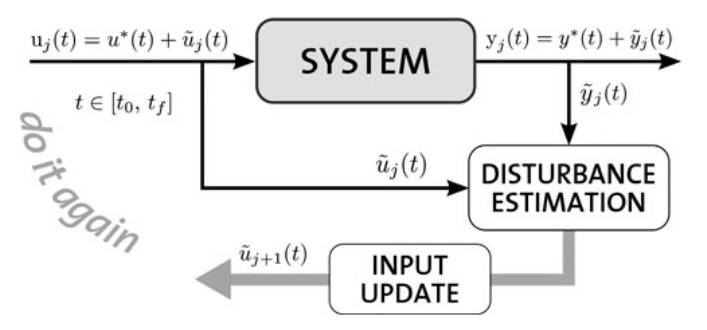
\includegraphics[scale=0.25]{ilc_framework}			
\caption{ILC Framework \cite{ILC_Angela}}
\end{figure}
\end{frame}
%
\section{Methodology}
%
\begin{frame}{Problem Setting}
\begin{itemize}
\item Problem: Continuous time trajectory tracking under the \emph{nonlinear} system dynamics: \pause
\end{itemize}
\begin{equation*}
\begin{aligned}
\dot{\state}(t) &= \mathbf{f}(\state(t),\sysInput(t)) \\
\observations(t) &= \mathbf{g(x(t))} 
\end{aligned}
\end{equation*}
\begin{itemize}
\item Goal: Track a reference trajectory $\traj(t), \ 0 \leq t \leq T \ $ by applying the control inputs $\sysInput^{*}(t)$. \pause
\item Use: Any trajectory generation algorithm~\footnote{See \cite{Zhang} for a spline-based method for differential-flat dynamics} that comes up with $\sysInput^{*}(t)$ %using a nominal model $\mathbf{f}_{nom}(\state(t),\sysInput(t))$
.\pause 
\end{itemize}
\end{frame}
%
\begin{frame}{Problem Setting}
\begin{itemize}	
\item However $\mathbf{f}$ is not known very well! \pause
\item We will fail to track $\traj(t)$ just by applying $\sysInput^{*}(t)$. \pause
\item We can use ILC to correct for deviations! \pause
\item We will follow the method of Sch\"{o}llig et al. \cite{ILC_Angela} in the following slides. 
\end{itemize}
\end{frame}
%
\subsection{Lifted vector representation}
%
\begin{frame}{Linearize Around Trajectory}
\begin{itemize}
\item Linearize model around trajectory: \pause
\end{itemize}
\begin{equation*}
\begin{aligned}
\dot{\tilde{\state}}(t) &= A(t)\tilde{\state}(t) + B(t)\tilde{\sysInput}(t) \\
\tilde{\observations}(t) &= C(t)\tilde{\state}(t) \\
\end{aligned}
\end{equation*} \pause
\begin{itemize}
\item The time variant matrices are: \pause
\linebreak
\end{itemize}
\begin{equation*}
\begin{aligned}
A(t) & = \at{\frac{\partial{\mathbf{f}}}{\partial{\state}}}{(\state^{*}(t),\sysInput^{*}(t))} \\
B(t) & = \at{\frac{\partial{\mathbf{f}}}{\partial{\observations}}}{(\state^{*}(t),\sysInput^{*}(t))} \\
C(t) & = \at{\frac{\partial{\mathbf{g}}}{\partial{\state}}}{\state^{*}(t)} \\
\end{aligned}
\end{equation*}
\end{frame}
%
\begin{frame}{Discretize linearized model}
\begin{itemize}
\item For k $\in \{ 0, 1, \ldots, N-1 \}$, \pause
\end{itemize}
\begin{equation*}
\begin{aligned}
\tilde{\state}(k+1) &= A_{D}(k)\tilde{\state}(k) + B_{D}(k)\tilde{\observations}(k) \\
\tilde{\observations}(k+1) &= C_{D}(k+1)\tilde{\state}(k+1)
\end{aligned}
\end{equation*}
\pause
\begin{itemize}
\item The discretized matrices can be found using: \pause
\linebreak
\end{itemize}
\begin{equation*}
\begin{aligned}
\exp^{h
\left[
\scalemath{0.5}{
\begin{array}{c|c}
A(k) & B(k) \\ \hline
0 & 0
\end{array}}\right]}
&= 
\left[
\begin{array}{c|c}
A_{D}(k) & B_{D}(k) \\ \hline
0 & I
\end{array}\right] \\
C_{D}(k) &= C(k)
\end{aligned}
\end{equation*}
\end{frame}
%
\begin{frame}{Lifted Vector Representation}
\begin{itemize}
\item Stack inputs together, $\liftedinput = (\tilde{\sysInput}(1), \ldots, \tilde{\sysInput}(N-1))$ to obtain the lifted vector form: \pause
\end{itemize}
\begin{equation*}
\begin{aligned}
\liftedstate &= F\liftedinput + \disturbance^{0} \\
\liftedobs &= G\liftedstate  
\end{aligned}
\end{equation*}
\pause
\begin{itemize}
\item where the submatrices are: \pause
\linebreak
\end{itemize}
\begin{equation*}
\begin{aligned}
F_{(i,j)} &= \left \{
\begin{array}{cc}
A_{D}(i-1)\ldots A_{D}(j)B_{D}(j-1), & j < i \\ 
B_{D}(j-1), & j = i \\
0, & j > i 
\end{array} \right. \\
G_{(i,j)} &= C_{D}
\end{aligned}
\end{equation*}
\end{frame}
%
\begin{frame}{Disturbance Model}
\begin{itemize}
\item The model for the evolution of disturbance over iterations: \pause
\linebreak
\end{itemize}
\begin{equation}
\begin{aligned}
\liftedstate_l &= F\liftedinput_l + \disturbance_l + \epsilon \\
\liftedobs_l &= G\liftedstate_l + \nu \\
\disturbance_l &= \disturbance_{l-1} + \omega_{l-1} \\
\epsilon &\sim \mathcal{N}(0,\Sigma_{\epsilon}) \\
\nu &\sim \mathcal{N}(0,\Sigma_{\nu}) \\
\omega &\sim \mathcal{N}(0,\Sigma_{\omega}) \\
\end{aligned}
\end{equation}
\end{frame}
%
\subsection{Disturbance Estimation}
%
\begin{frame}{Disturbance Estimation}
\begin{itemize}
\item The disturbance model \pause
\linebreak
\end{itemize}
\begin{equation}
\begin{aligned}
\disturbance_l &= \disturbance_{l-1} + \omega_{l-1} \\
\liftedobs_l &= G\disturbance_l + GF\liftedinput_l + \eta \\
\omega &\sim \mathcal{N}(0,\Sigma_{\omega}) \\
\eta &\sim \mathcal{N}(0,\Sigma_{\eta} = G\Sigma_{\epsilon}G^{\mathrm{T}} + \Sigma_{\nu}) \\
\end{aligned}
\end{equation}
\pause
\begin{itemize}
\item is estimated with a Kalman filter. \pause
\end{itemize}
\end{frame}
%
\begin{frame}{Kalman Filter}
\begin{itemize}
\item Kalman filter equations: \pause
\end{itemize}
\begin{equation}
\begin{aligned}
\bar{\mu}_t &= A_t\mu_{t-1} + B_t u_t \\
\bar{\Sigma}_t &= A_t\Sigma_{t-1}A_t^{\mathrm{T}} + \Sigma_{\omega} \\
K_t &= \bar{\Sigma}_t C_t^{\mathrm{T}}(C_t \bar{\Sigma}_t C_t^{\mathrm{T}} + \Sigma_{\eta})^{-1} \\
\mu_t &= \bar{\mu}_t + K_t (y_t - C_t \bar{\mu}_t) \\
\Sigma_t &= (I - K_t C_t)\bar{\Sigma}_t
\end{aligned}
\end{equation}
\pause
\begin{itemize}
\item for $A_t = I$, $B_t = 0$ become: \pause
\linebreak
\end{itemize}
\begin{equation}
\begin{aligned}
\hat{\disturbance}_l &= \hat{\disturbance}_{l-1} + K_{l}(y_l - G\hat{\disturbance}_{l-1} - GF\liftedinput_l) \\
\bar{\Sigma}_l &= \Sigma_{l-1} + \Sigma_{\omega} \\
K_l &= \bar{\Sigma}_l G^{\mathrm{T}}(G\bar{\Sigma}_l G^{\mathrm{T}} + \Sigma_{\eta})^{-1} \\
\Sigma_{l} &= (I - K_l G)\bar{\Sigma}_l
\end{aligned}
\end{equation}
\end{frame}
%
\subsection{Input update}
%
\begin{frame}{Input update}
\begin{itemize}
\item The goal is to compensate for the disturbances by updating $\liftedinput$ adequately: $\min_{\liftedinput_{l+1}} \mathbb{E}[\liftedstate_{l+1}| \liftedobs_1, \ldots, \liftedobs_l] = \min_{\liftedinput_{l+1}} F\liftedinput_{l+1} + \hat{\disturbance}_l$ \pause 
\item We can also add (lifted vector) constraints in a convex optimization framework: \pause
\end{itemize}
\begin{equation}
\begin{aligned}
\liftedinput_{l+1} = \arg\min_{u} &\|F\liftedinput + \hat{\disturbance}_l \|_{2} \\
& \text{s.t.} \\
L\liftedinput & \leq q
\end{aligned}
\end{equation}
\pause
\begin{itemize}
\item $\sysInput(t) = \sysInput^{*}(t) + \liftedinput_{l+1}(t)$
\end{itemize}
\end{frame}
%
\section{Example}
\begin{frame}{Example}
\begin{itemize}
\item Wind disturbance during quadrocopter operation. \pause
\item 2D Quadrocopter dynamics modified as follows: \pause
\end{itemize}
\begin{equation}
\begin{aligned}
\ddot{y} &= -f_{\mathrm{coll}} \sin\phi + P_{wind} A sin(\theta + \phi) cos \theta \\
\ddot{z} &=  f_{\mathrm{coll}}\cos\phi - g + P_{wind} A sin(\theta + \phi) sin \theta \\
\dot{\phi} &= \omega_{x}
\end{aligned}
\end{equation}
\begin{figure}
\center
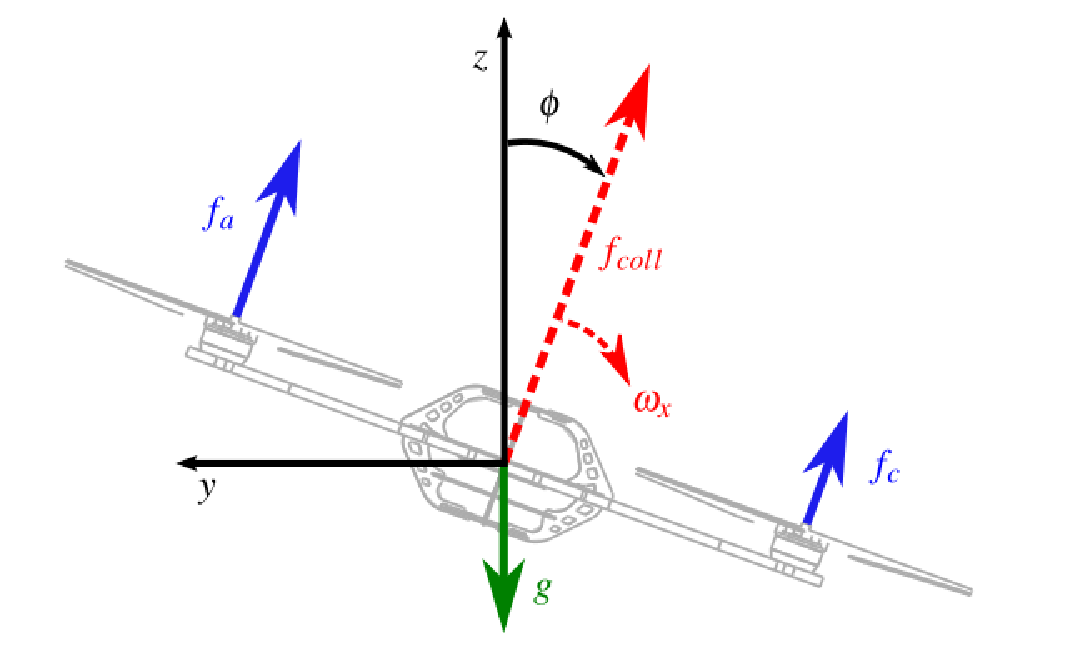
\includegraphics[scale=0.25]{quadrocopter}			
\caption{2D Quadrocopter model}
\end{figure}
\end{frame}
%
\begin{frame}{Example}
\begin{figure}[!htb]
\minipage{0.5\textwidth}
  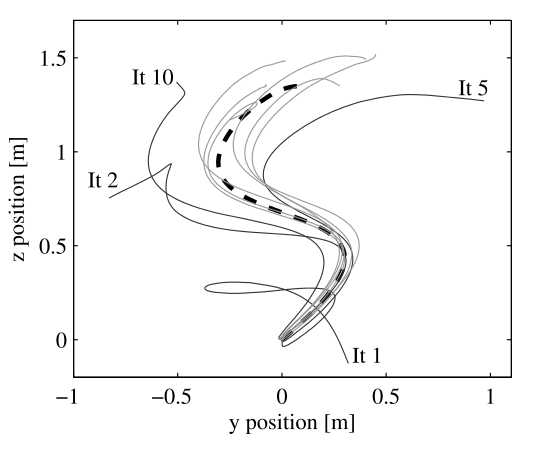
\includegraphics[width=\linewidth]{ilc.png}
  \caption{Learning an S-shaped trajectory}
\endminipage\hfill
\minipage{0.5\textwidth}
  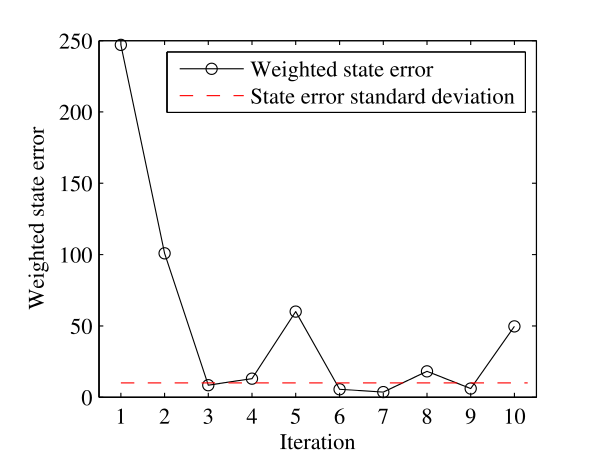
\includegraphics[width=\linewidth]{ilc_error.png}
  \caption{Errors vs. iterations}
\endminipage
\end{figure}
\end{frame}
%
\section{Analysis}
%
\begin{frame}{Analysis of the method}
\begin{itemize}
\item Works great, especially with a feedback controller! \pause
\item No guarantee of stability! \pause
\item No guarantee of convergence! \pause
	\begin{itemize}
	\item Modelling disturbances $\disturbance_l$ as `random walk' is not accurate! \pause
	\item $\liftedstate_l = F_{\mathrm{nom}}\liftedinput_l + \Delta F \liftedinput_l + \epsilon$ \pause
	\item Is it possible to estimate $\Delta F$ from the inputs $(\sysInput_1, \ldots, \sysInput_l)$ and output trajectories $(\observations_1, \ldots, \observations_l)$? \pause
	\end{itemize}
\item In other nonlinear ILC approaches \cite{Xu}, contraction mappings and Lyapunov analysis is used to show convergence and stability.
\end{itemize}
\end{frame}
%
%
%\section{Other ILC Approaches}
%
\section{Combining ILC with ProMPs for Transfer Learning}
%
\begin{frame}{Transfer Learning with ProMPs}
\begin{itemize}
\item ILC has to learn from scratch each time a trajectory changes! \pause
\item Guilherme and Geri's idea: \pause
\begin{itemize}
\item Train a ProMP with all of the ILC iterations as demonstrations. \pause
\item Generalize to different endpoints or trajectories.
\end{itemize}
\end{itemize}
\end{frame}	
%
\begin{frame}{Conclusion}
\begin{itemize}
\item Thank you for listening!
\end{itemize}
\end{frame}	
%
\section{References}
\begin{frame}[allowframebreaks]{References}
\def\newblock{\hskip .11em plus .33em minus .07em}
\bibliographystyle{alpha}
\bibliography{myReferences} % file name of the bibtex
\end{frame}
%

%
% End of slides
\end{document} 